\PassOptionsToPackage{unicode=true}{hyperref} % options for packages loaded elsewhere
\PassOptionsToPackage{hyphens}{url}
\PassOptionsToPackage{dvipsnames,svgnames*,x11names*}{xcolor}
%
\documentclass[ignorenonframetext,hyperref,x11names,UTF8]{beamer}
\setbeamertemplate{caption}[numbered]
\setbeamertemplate{caption label separator}{: }
\setbeamercolor{caption name}{fg=normal text.fg}
\beamertemplatenavigationsymbolsempty
\usepackage{lmodern}
\usepackage{amssymb,amsmath}
\usepackage{ifxetex,ifluatex}
\usepackage{fixltx2e} % provides \textsubscript
\ifnum 0\ifxetex 1\fi\ifluatex 1\fi=0 % if pdftex
  \usepackage[T1]{fontenc}
  \usepackage[utf8]{inputenc}
  \usepackage{textcomp} % provides euro and other symbols
\else % if luatex or xelatex
  \usepackage{unicode-math}
  \defaultfontfeatures{Ligatures=TeX,Scale=MatchLowercase}
\fi
\usetheme[]{Singapore}
\usefonttheme{structurebold}
% use upquote if available, for straight quotes in verbatim environments
\IfFileExists{upquote.sty}{\usepackage{upquote}}{}
% use microtype if available
\IfFileExists{microtype.sty}{%
\usepackage[]{microtype}
\UseMicrotypeSet[protrusion]{basicmath} % disable protrusion for tt fonts
}{}
\IfFileExists{parskip.sty}{%
\usepackage{parskip}
}{% else
\setlength{\parindent}{0pt}
\setlength{\parskip}{6pt plus 2pt minus 1pt}
}
\usepackage{xcolor}
\usepackage{hyperref}
\hypersetup{
            pdftitle={空间广义线性混合效应模型及其应用},
            pdfauthor={学生:黄湘云导师:李再兴},
            colorlinks=true,
            linkcolor=SpringGreen4,
            citecolor=Blue,
            urlcolor=Blue,
            breaklinks=true}
\urlstyle{same}  % don't use monospace font for urls
\newif\ifbibliography
% Prevent slide breaks in the middle of a paragraph:
\widowpenalties 1 10000
\raggedbottom
\setlength{\emergencystretch}{3em}  % prevent overfull lines
\providecommand{\tightlist}{%
  \setlength{\itemsep}{0pt}\setlength{\parskip}{0pt}}
\setcounter{secnumdepth}{0}

% set default figure placement to htbp
\makeatletter
\def\fps@figure{htbp}
\makeatother

\usepackage{ctex}
\usecolortheme[named=SpringGreen4]{structure}
\usepackage[default]{sourcesanspro}
\usepackage[]{natbib}
\bibliographystyle{apalike}

\title{空间广义线性混合效应模型及其应用}
\providecommand{\subtitle}[1]{}
\subtitle{2018届硕士学位论文答辩}
\author{学生:黄湘云\and 导师:李再兴}
\providecommand{\institute}[1]{}
\institute{中国矿业大学(北京)\and 理学院}
\date{\today}

\begin{document}
\frame{\titlepage}

\begin{frame}
\tableofcontents[hideallsubsections]
\end{frame}
\section{引言}

\begin{frame}{R Markdown}

This is an R Markdown presentation \citep{bookdown2016CRC}. Markdown is
a simple formatting syntax for authoring HTML, PDF, and MS Word
documents. For more details on using R Markdown see
\url{http://rmarkdown.rstudio.com}.

When you click the \textbf{Knit} button a document will be generated
that includes both content as well as the output of any embedded R code
chunks within the document.

\end{frame}

\begin{frame}{Slide with Bullets}

\begin{itemize}
\tightlist
\item
  Bullet 1
\item
  Bullet 2
\item
  Bullet 3
\end{itemize}

\end{frame}

\section{算法}

\begin{frame}[fragile]{Slide with R Output}

\begin{verbatim}
summary(cars)
##      speed           dist       
##  Min.   : 4.0   Min.   :  2.00  
##  1st Qu.:12.0   1st Qu.: 26.00  
##  Median :15.0   Median : 36.00  
##  Mean   :15.4   Mean   : 42.98  
##  3rd Qu.:19.0   3rd Qu.: 56.00  
##  Max.   :25.0   Max.   :120.00
\end{verbatim}

\end{frame}

\begin{frame}[fragile]{Slide with Plot}

\begin{verbatim}
plot(pressure)
\end{verbatim}

\begin{center}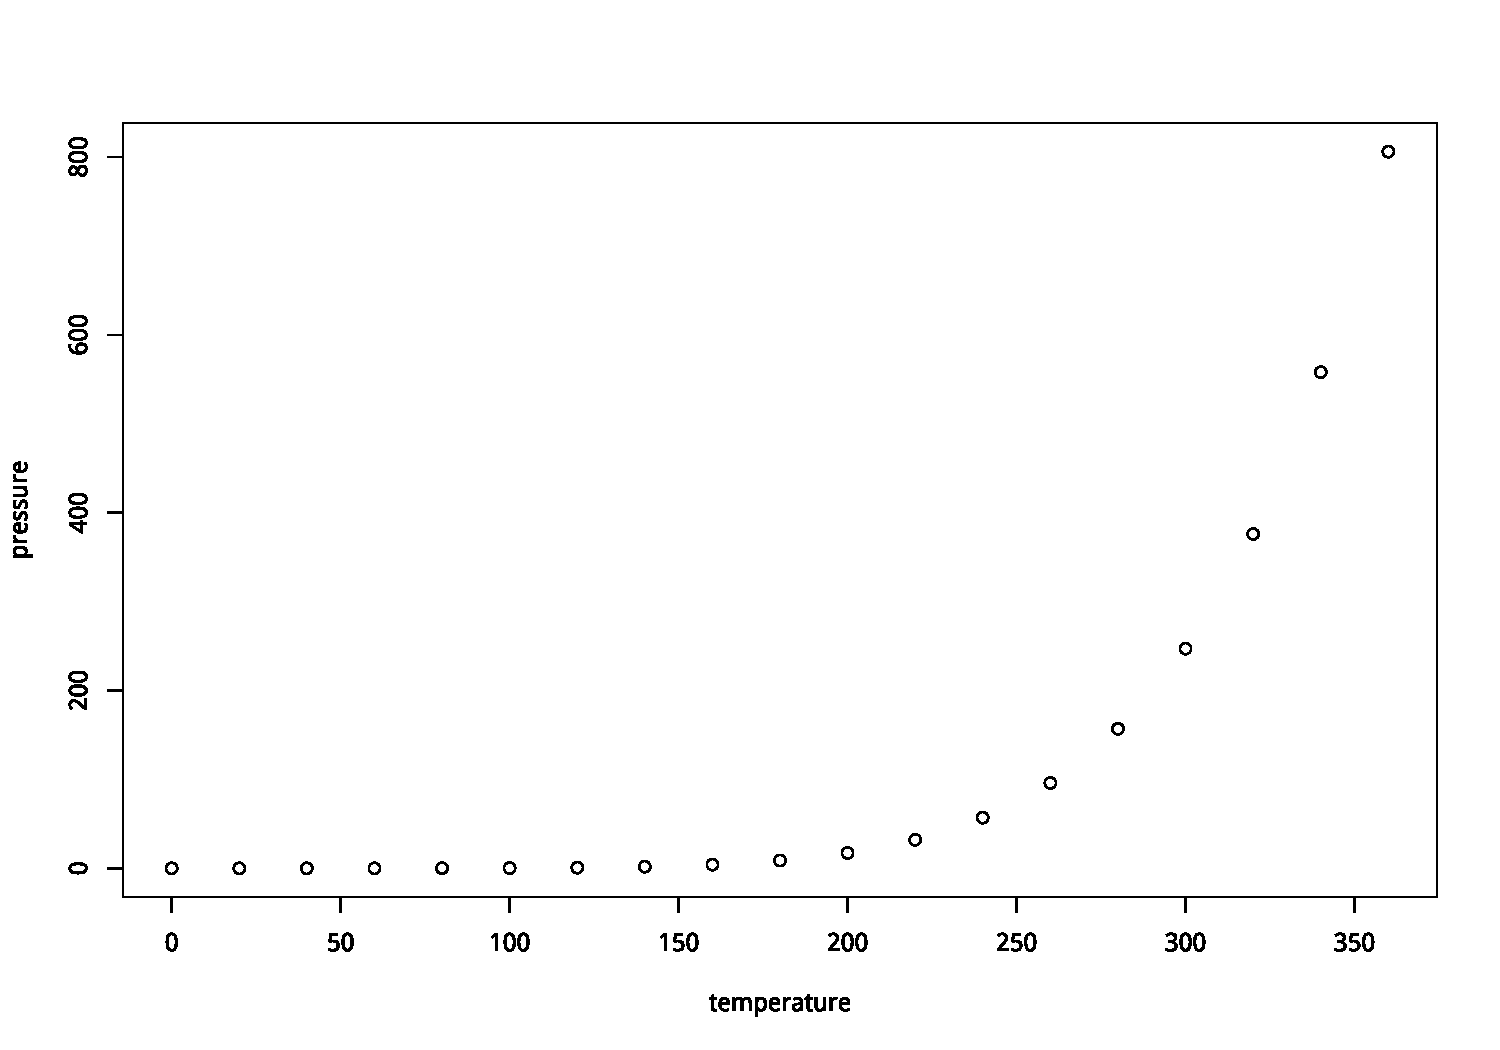
\includegraphics[width=.7\textwidth]{oral-defense_files/figure-beamer/pressure-1} \end{center}

\end{frame}

\begin{frame}{语法高亮}

\end{frame}

\renewcommand\refname{参考文献}
\begin{frame}[allowframebreaks]{参考文献}
\bibliographytrue
\bibliography{refer.bib}
\end{frame}

\end{document}
